\documentclass[12pt, titlepage]{article}

\usepackage{fullpage}
\usepackage[round]{natbib}
\usepackage{multirow}
\usepackage{booktabs}
\usepackage{tabularx}
\usepackage{graphicx}
\usepackage{float}
\usepackage{hyperref}
\hypersetup{
    colorlinks,
    citecolor=blue,
    filecolor=black,
    linkcolor=red,
    urlcolor=blue
}

\input{../../Comments}
\input{../../Common}

\newcounter{acnum}
\newcommand{\actheacnum}{AC\theacnum}
\newcommand{\acref}[1]{AC\ref{#1}}

\newcounter{ucnum}
\newcommand{\uctheucnum}{UC\theucnum}
\newcommand{\uref}[1]{UC\ref{#1}}

\newcounter{mnum}
\newcommand{\mthemnum}{M\themnum}
\newcommand{\mref}[1]{M\ref{#1}}

\begin{document}

\title{Module Guide for Re-ProtGNN} 
\author{\authname}
\date{\today}

\maketitle

\pagenumbering{roman}

\section{Revision History}

\begin{tabularx}{\textwidth}{p{3cm}p{2cm}X}
\toprule {\bf Date} & {\bf Version} & {\bf Notes}\\
\midrule
Mar 19, 2025 & 1.0 & First Draft\\
\bottomrule
\end{tabularx}

\newpage

\section{Reference Material}

This section records information for easy reference.

\subsection{Abbreviations and Acronyms}

\renewcommand{\arraystretch}{1.2}
\begin{tabular}{l l} 
  \toprule		
  \textbf{symbol} & \textbf{description}\\
  \midrule 
  AC & Anticipated Change\\
  DAG & Directed Acyclic Graph \\
  M & Module \\
  MG & Module Guide \\
  OS & Operating System \\
  R & Requirement\\
  SC & Scientific Computing \\
  SRS & Software Requirements Specification\\
  \progname & Explanation of program name\\
  UC & Unlikely Change \\
  Re-ProtGNN & Re-implementation of the Prototype-based Graph Neural Network model \\
  \bottomrule
\end{tabular}\\

\newpage

\tableofcontents

\listoftables

\listoffigures

\newpage

\pagenumbering{arabic}

\section{Introduction}

Decomposing a system into modules is a commonly accepted approach to developing
software.  A module is a work assignment for a programmer or programming
team~\citep{ParnasEtAl1984}.  We advocate a decomposition
based on the principle of information hiding~\citep{Parnas1972a}.  This
principle supports design for change, because the ``secrets'' that each module
hides represent likely future changes.  Design for change is valuable in SC,
where modifications are frequent, especially during initial development as the
solution space is explored.  

Our design follows the rules layed out by \citet{ParnasEtAl1984}, as follows:
\begin{itemize}
\item System details that are likely to change independently should be the
  secrets of separate modules.
\item Each data structure is implemented in only one module.
\item Any other program that requires information stored in a module's data
  structures must obtain it by calling access programs belonging to that module.
\end{itemize}

After completing the first stage of the design, the Software Requirements
Specification (SRS), the Module Guide (MG) is developed~\citep{ParnasEtAl1984}. The MG
specifies the modular structure of the system and is intended to allow both
designers and maintainers to easily identify the parts of the software.  The
potential readers of this document are as follows:

\begin{itemize}
\item New project members: This document can be a guide for a new project member
  to easily understand the overall structure and quickly find the
  relevant modules they are searching for.
\item Maintainers: The hierarchical structure of the module guide improves the
  maintainers' understanding when they need to make changes to the system. It is
  important for a maintainer to update the relevant sections of the document
  after changes have been made.
\item Designers: Once the module guide has been written, it can be used to
  check for consistency, feasibility, and flexibility. Designers can verify the
  system in various ways, such as consistency among modules, feasibility of the
  decomposition, and flexibility of the design.
\end{itemize}

The rest of the document is organized as follows. Section
\ref{SecChange} lists the anticipated and unlikely changes of the software
requirements. Section \ref{SecMH} summarizes the module decomposition that
was constructed according to the likely changes. Section \ref{SecConnection}
specifies the connections between the software requirements and the
modules. Section \ref{SecMD} gives a detailed description of the
modules. Section \ref{SecTM} includes two traceability matrices. One checks
the completeness of the design against the requirements provided in the SRS. The
other shows the relation between anticipated changes and the modules. Section
\ref{SecUse} describes the use relation between modules.

\section{Anticipated and Unlikely Changes} \label{SecChange}

This section lists possible changes to the system. According to the likeliness
of the change, the possible changes are classified into two
categories. Anticipated changes are listed in Section \ref{SecAchange}, and
unlikely changes are listed in Section \ref{SecUchange}.

\subsection{Anticipated Changes} \label{SecAchange}

Anticipated changes are the source of the information that is to be hidden
inside the modules. Ideally, changing one of the anticipated changes will only
require changing the one module that hides the associated decision. The approach
adapted here is called design for
change.

\begin{description}
\item[\refstepcounter{acnum} \actheacnum \label{acHardware}:] The specific
  hardware on which the software is running.
\item[\refstepcounter{acnum} \actheacnum \label{acConfig}:]  The values of hyperparameters used for model architecture, optimization, and explanation.
\item[\refstepcounter{acnum} \actheacnum \label{acInput}:] The format of the
  initial input data.
\item[\refstepcounter{acnum} \actheacnum \label{acControl}:] The pipeline stages of the system, such as adding a stage for visualizing model explanations after training.

\item[\refstepcounter{acnum} \actheacnum \label{acTrain}:] The optimization algorithm used in training, such as changing from Adam to Stochastic Gradient Descent.
\item[\refstepcounter{acnum} \actheacnum \label{acInf}:] The prediction postprocessing method when doing inference. 
\item[\refstepcounter{acnum} \actheacnum \label{acModel}:] The activation function of the model.
\item[\refstepcounter{acnum} \actheacnum \label{acExp}:] The method by which prototype vectors are mapped to real subgraphs.
\item[\refstepcounter{acnum} \actheacnum \label{acVil}:] The visualization techniques for presenting model outputs and explanations.
\item[\refstepcounter{acnum} \actheacnum \label{acTorch}:] The loss function used for model training.
\item[\refstepcounter{acnum} \actheacnum \label{acPyG}:] The batching mechanism for graph data.
\item[\refstepcounter{acnum} \actheacnum \label{acGUI}:] The figure rendering strategy.
\end{description}

\subsection{Unlikely Changes} \label{SecUchange}

The module design should be as general as possible. However, a general system is
more complex. Sometimes this complexity is not necessary. Fixing some design
decisions at the system architecture stage can simplify the software design. If
these decision should later need to be changed, then many parts of the design
will potentially need to be modified. Hence, it is not intended that these
decisions will be changed.

\begin{description}
\item[\refstepcounter{ucnum} \uctheucnum \label{ucIO}:] Input/Output devices
  (Input: File and/or Keyboard, Output: File, Memory, and/or Screen).
\item[\refstepcounter{ucnum} \uctheucnum \label{ucI1}:] The use of \texttt{Tensor} from PyTorch for numerical computation, including matrix operations and gradient-based learning.
\item[\refstepcounter{ucnum} \uctheucnum \label{ucI2}:] The use of PyTorch Geometric libraries for handling graph data, including the \texttt{Data} object, which encapsulates node features, edge indices, and optionally labels, to represent individual graphs, and the \texttt{DataLoader}, which provides mini-batch support for training and inference workflows.
\end{description}

\section{Module Hierarchy} \label{SecMH}

This section provides an overview of the module design. Modules are summarized
in a hierarchy decomposed by secrets in Table \ref{TblMH}. The modules listed
below, which are leaves in the hierarchy tree, are the modules that will
actually be implemented.

\begin{description}
\item [\refstepcounter{mnum} \mthemnum \label{mHH}:]Hardware-Hiding Module
\item [\refstepcounter{mnum} \mthemnum \label{mConfig}:]Configuration Module
\item [\refstepcounter{mnum} \mthemnum \label{mInput}:] Input Format Module
\item [\refstepcounter{mnum} \mthemnum \label{mControl}:] Control Module
\item [\refstepcounter{mnum} \mthemnum \label{mTrain}:] Training Module
\item [\refstepcounter{mnum} \mthemnum \label{mVil}:] Output Visualization Module
\item [\refstepcounter{mnum} \mthemnum \label{mModel}:] Model Module
\item [\refstepcounter{mnum} \mthemnum \label{mInf}:] Inference Module
\item [\refstepcounter{mnum} \mthemnum \label{mExp}:] Explanation Module
\item [\refstepcounter{mnum} \mthemnum \label{mTorch}:] PyTorch Module
\item [\refstepcounter{mnum} \mthemnum \label{mPyG}:] PyTorch Geometric Module
\item [\refstepcounter{mnum} \mthemnum \label{mGUI}:] GUI Module

\end{description}


\begin{table}[h!]
\centering
\begin{tabular}{p{0.3\textwidth} p{0.6\textwidth}}
\toprule
\textbf{Level 1} & \textbf{Level 2}\\
\midrule

{Hardware-Hiding Module} & ~ \\
\midrule

\multirow{4}{0.3\textwidth}{Behaviour-Hiding Module} 
& Configuration Module\\
& Input Format Module\\
& Control Module\\
& Training Module\\
& Output Visualization Module\\
\midrule

\multirow{3}{0.3\textwidth}{Software Decision Module} & {Model Module}\\
& Inference Module\\
& Explanation Module\\
& PyTorch Module\\
& PyTorch Geometric Module\\
& GUI Module\\
\bottomrule

\end{tabular}
\caption{Module Hierarchy}
\label{TblMH}
\end{table}

\section{Connection Between Requirements and Design} \label{SecConnection}

The design of the system is intended to satisfy the requirements developed in
the SRS. In this stage, the system is decomposed into modules. The connection
between requirements and modules is listed in Table~\ref{TblRT}.

\section{Module Decomposition} \label{SecMD}

Modules are decomposed according to the principle of ``information hiding''
proposed by \citet{ParnasEtAl1984}. The \emph{Secrets} field in a module
decomposition is a brief statement of the design decision hidden by the
module. The \emph{Services} field specifies \emph{what} the module will do
without documenting \emph{how} to do it. For each module, a suggestion for the
implementing software is given under the \emph{Implemented By} title. If the
entry is \emph{OS}, this means that the module is provided by the operating
system or by standard programming language libraries.  \emph{Re-ProtGNN} means the
module will be implemented by the Re-ProtGNN software.

Only the leaf modules in the hierarchy have to be implemented. If a dash
(\emph{--}) is shown, this means that the module is not a leaf and will not have
to be implemented.

\subsection{Hardware Hiding Modules (\mref{mHH})}

\begin{description}
\item[Secrets:]The data structure and algorithm used to implement the virtual
  hardware.
\item[Services:]Serves as a virtual hardware used by the rest of the
  system. This module provides the interface between the hardware and the
  software. So, the system can use it to display outputs or to accept inputs.
\item[Implemented By:] OS
\end{description}

\subsection{Behaviour-Hiding Module}

\begin{description}
\item[Secrets:]The contents of the required behaviours.
\item[Services:]Includes programs that provide externally visible behaviour of
  the system as specified in the software requirements specification (SRS)
  documents. This module serves as a communication layer between the
  hardware-hiding module and the software decision module. The programs in this
  module will need to change if there are changes in the SRS.
\item[Implemented By:] --
\end{description}


\subsubsection{Configuration Module (\mref{mConfig})}

\begin{description}
\item[Secrets:] The internal definitions of experiment configuration classes, including dataset selection, model hyperparameters, training schedule, explanation strategy parameters, and reward computation settings.

\item[Services:] Exports user-defined hyperparameter instances and global configuration objects (\texttt{data\_args}, \texttt{model\_args}, \texttt{train\_args}, etc.) for consistent access across modules.

\item[Implemented By:] Re-ProtGNN

\item[Type of Module:] Library

\end{description}


\subsubsection{Input Format Module (\mref{mInput})}

\begin{description}
\item[Secrets:]The format of the input graph datasets.
\item[Services:]Loads and parses datasets into standardized graph representations using PyTorch Geometric data structures.
\item[Implemented By:] Re-ProtGNN
\item[Type of Module:] Library
\end{description}

\subsubsection{Control Module (\mref{mControl})}

\begin{description}
\item[Secrets:]: The execution flow of the system.

\item[Services:]Manages the training, inference, and visualization processes.
\item[Implemented By:] Re-ProtGNN
\item[Type of Module:] Main program
\end{description}

\subsubsection{Training Module
 (\mref{mTrain})}

\begin{description}
\item[Secrets:] The optimization techniques used in training.

\item[Services:] Trains the ProtGNN model using supervised and prototype-based losses, and records the loss value and accuracy for each epoch in log files.

\item[Implemented By:] Re-ProtGNN
\item[Type of Module:] Library
\end{description}

\subsubsection{Output Visualization Module
 (\mref{mVil})}

\begin{description}
\item[Secrets:] How model prediction outputs and explanations are visualized.
\item[Services:] Generates visual representations of explanations and outputs prediction accuracy.

\item[Implemented By:] Re-ProtGNN
\item[Type of Module:] Library
\end{description}




\subsection{Software Decision Module}

\begin{description}
\item[Secrets:] The design decision based on mathematical theorems, physical
  facts, or programming considerations. The secrets of this module are
  \emph{not} described in the SRS.
\item[Services:] Includes data structure and algorithms used in the system that
  do not provide direct interaction with the user. 
  % Changes in these modules are more likely to be motivated by a desire to
  % improve performance than by externally imposed changes.
\item[Implemented By:] --
\end{description}

\subsubsection{Model Module
 (\mref{mModel})}

\begin{description}
\item[Secrets:] The architecture of the Re-ProtGNN model.
\item[Services:] Defines the parameters and structural design of the Re-ProtGNN model.
\item[Implemented By:] Re-ProtGNN
\item[Type of Module:] Abstract Data Type
\end{description}


\subsubsection{Inference Module
 (\mref{mInf})}

\begin{description}
\item[Secrets:] The details of how inference is conducted using the trained model.

\item[Services:] Runs inference in evaluation mode and outputs predictions.

\item[Implemented By:] Re-ProtGNN
\item[Type of Module:] Library
\end{description}


\subsubsection{Explanation Module
 (\mref{mExp})}

\begin{description}
\item[Secrets:] How prototype vectors are mapped onto real subgraphs.

\item[Services:] Updates prototypes to be near real subgraph embeddings, improving interpretability.

\item[Implemented By:] Re-ProtGNN
\item[Type of Module:] Library
\end{description}


\subsubsection{PyTorch Module (\mref{mTorch})}
\begin{description} 
\item[Secrets:] Internal tensor operations, optimizers, and loss functions used during training and inference. \item[Services:] Provides tensor-based computation (e.g., matrix operations), gradient propagation, and loss/optimizer routines that are foundational for training deep learning models. 
\item[Implemented By:] PyTorch Library 
\item[Type of Module:] External Library \end{description}

\subsubsection{PyTorch Geometric Module (\mref{mPyG})}
\begin{description} 
\item[Secrets:] Graph representations, batch processing, and transformation utilities specific to graph-structured data. \item[Services:] Provides data structures (\texttt{Data}, \texttt{Dataset}, \texttt{DataLoader}) and utility functions (e.g., \texttt{to\_networkx}) for handling graph input/output and mini-batching. 
\item[Implemented By:] PyTorch Geometric Library 
\item[Type of Module:] External Library \end{description}

\subsubsection{GUI Module (\mref{mGUI})}
\begin{description} 
\item[Secrets:] The rendering and saving process of images used to display predictions and subgraph explanations. \item[Services:] Supports figure creation and rendering via Matplotlib.
\item[Implemented By:] Matplotlib Library 
\item[Type of Module:] External Library \end{description}




\section{Traceability Matrix} \label{SecTM}

This section shows two traceability matrices: between the modules and the
requirements and between the modules and the anticipated changes.

% the table should use mref, the requirements should be named, use something
% like fref
\begin{table}[H]
\centering
\begin{tabular}{p{0.2\textwidth} p{0.6\textwidth}}
\toprule
\textbf{Req.} & \textbf{Modules}\\
\midrule
R1 & \mref{mHH}, \mref{mInput}, \mref{mControl}, \mref{mTorch}, \mref{mPyG}\\
R2 & \mref{mConfig}, \mref{mTrain}, \mref{mModel}, \mref{mTorch}, \mref{mGUI}\\
R3 & \mref{mVil}, \mref{mInf}, \mref{mExp}, \mref{mTorch} \\
\bottomrule
\end{tabular}
\caption{Trace Between Requirements and Modules}
\label{TblRT}
\end{table}

\begin{table}[H]
\centering
\begin{tabular}{p{0.2\textwidth} p{0.6\textwidth}}
\toprule
\textbf{AC} & \textbf{Modules}\\
\midrule
\acref{acHardware} & \mref{mHH}\\
\acref{acConfig} & \mref{mConfig}\\
\acref{acInput} & \mref{mInput}\\
\acref{acControl} & \mref{mControl}\\
\acref{acTrain} & \mref{mTrain}\\
\acref{acInf} & \mref{mInf}\\
\acref{acModel} & \mref{mModel}\\
\acref{acExp} & \mref{mExp}\\
\acref{acVil} & \mref{mVil}\\
\acref{acTorch} & \mref{acTorch}\\
\acref{acPyG} & \mref{acPyG}\\
\acref{acGUI} & \mref{acGUI}\\
\bottomrule
\end{tabular}
\caption{Trace Between Anticipated Changes and Modules}
\label{TblACT}
\end{table}

\section{Use Hierarchy Between Modules} \label{SecUse}

In this section, the uses hierarchy between modules is
provided. \citet{Parnas1978} said of two programs A and B that A {\em uses} B if
correct execution of B may be necessary for A to complete the task described in
its specification. That is, A {\em uses} B if there exist situations in which
the correct functioning of A depends upon the availability of a correct
implementation of B.  Figure \ref{FigUH} illustrates the use relation between
the modules. It can be seen that the graph is a directed acyclic graph
(DAG). Each level of the hierarchy offers a testable and usable subset of the
system, and modules in the higher level of the hierarchy are essentially simpler
because they use modules from the lower levels.


\begin{figure}[H]
\centering
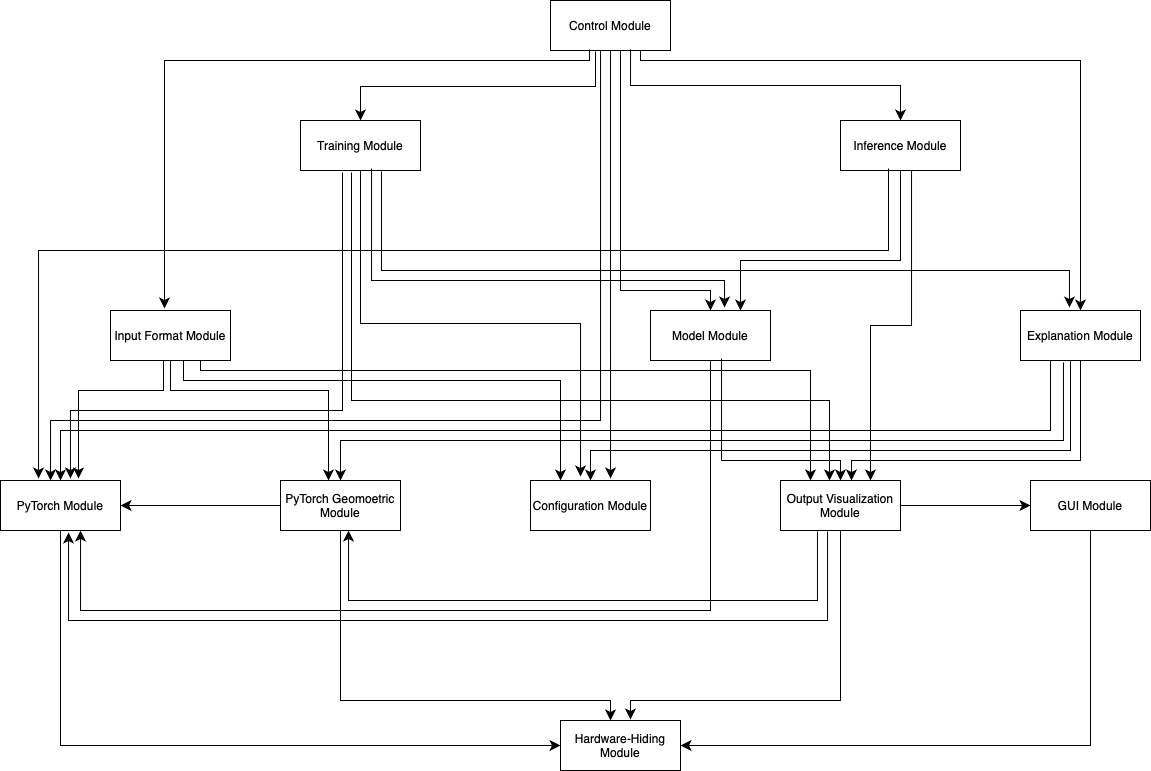
\includegraphics[width=1\textwidth]{UsesHierarchy.png}
\caption{Use hierarchy among modules}
\label{FigUH}
\end{figure}

%\section*{References}

\section{User Interfaces}

The user interface for the Re-ProtGNN system will be a terminal-based interface. Users will interact with the system by running commands from the terminal. Input graph datasets must be placed in a specified input folder, and the system will automatically process them through the training and inference pipeline. Explanations will be generated as image files and saved to a designated output folder, along with prediction results and logs stored in a structured log file.

\section{Design of Communication Protocols}

Not applicable.

\section{Timeline}

Please refer to \href{https://github.com/Yuanqi-X/Re-ProtGNN/tree/main}{Github}.

\bibliographystyle {plainnat}
\bibliography{../../../refs/References}
%\bibliography{refs/References}

\newpage{}

\end{document}
